\documentclass[9pt]{beamer}

% --- Packages ---
\usepackage{amsmath, amssymb}
\usepackage{bm}
% (Optional) compile with XeLaTeX/LuaLaTeX for fonts
\usepackage{fontspec}
\setmainfont{Times New Roman}
\usepackage{unicode-math}

\usepackage{tikz}
\usetikzlibrary{arrows.meta, positioning, decorations.pathreplacing, calc, fit, backgrounds, patterns}

\usepackage{graphicx}
% resolve figures whether the deck is compiled from draft/ or from draft/slide/
\graphicspath{{figures/}{../figures/}}

\setbeamertemplate{footline}[frame number]
\setbeamertemplate{navigation symbols}{}
\setbeamertemplate{caption}{\insertcaption}

% color shorthands
\definecolor{accent}{RGB}{0,90,160}
\definecolor{invest}{RGB}{200,70,30}
\definecolor{shockc}{RGB}{20,140,90}

\title{Investment Demand Shock and Business Cycle}
\subtitle{A Bayesian estimation of a DSGE model}
\author{Li Xuanguang}
\date{\today}

\begin{document}

\begin{frame}
	\titlepage
	\vspace{-1em}
\end{frame}

\begin{frame}{Motivation}
	%content: motivation
	\begin{itemize}
		\item \textbf{Justiniano, Primiceri and Tambalotti (2010):} an estimated DSGE attributes a large share of U.S.\ fluctuations to a \textbf{investment-specific technology (IST) shock} ($K_{t+1}=(1-\delta)K_t+\mu_{s,t}I_t$).
		\item \textbf{The comovement puzzle:} IST shocks struggle to reproduce the joint positive comovement of consumption, investment, and inflation seen in the data.
		\item \textbf{Nirei and Ragot (2025):} proposed an \textbf{investment demand shock}, which can generate this comovement, but lacks empirical test.
	\end{itemize}
	\vspace{0.5em}
	\begin{block}{This paper}
		Estimate a DSGE model with both an IST shock and an investment demand shock to quantify how important the investment demand shock is for the U.S.\ business cycle.
	\end{block}
\end{frame}




\begin{frame}{Investment demand shock and its origin}
	Reduced-form \textbf{investment demand (ID) shock}:
	\[
		I_t=\mu_{d,t}\,I_t^{*},\qquad
		\ln\mu_{d,t}=(1-\rho_d)\ln\mu_d+\rho_d\ln\mu_{d,t-1}+\varepsilon_{d,t}.
	\]

	A toy New-Keynesian model with \textbf{lumpy investment assumption}, 
	$$i_{j,t}\in\{0,\ (\lambda-1)(1-\delta)k_{j,t}\}.$$

	\begin{columns}[T,onlytextwidth]
		\column{0.6\textwidth}
		\begin{itemize}
			\item Invest iff future capital below a threshold,
			$$k^{*}_{j,t+1}=a_{j,t+1}^{\,\eta-1}\Phi_t\,Y_{t+1}.$$
			\item Decision rule in terms of current capital:
			$$ i_{j,t}=
			\begin{cases}
				(\lambda-1)(1-\delta)k_{j,t}, \, k_{j,t}<\frac{k^{*}_{j,t+1}}{1-\delta}\\
				0,\, \text{otherwise}
			\end{cases}
			$$
		\end{itemize}

		\column{0.4\textwidth}
		
		\vspace{0.5em}

		\centering
		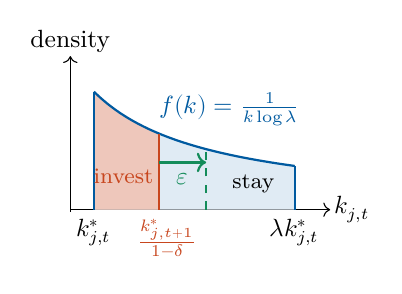
\begin{tikzpicture}[xscale=1.5,yscale=1.5]
			% axes
			\draw[->] (0.8,0) -- (3.0,0) node[right,font=\small,inner sep=1.5pt]{$k_{j,t}$};
			\draw[->] (0.8,-0.02) -- (0.8,1.3) node[above,font=\small,inner sep=1pt]{density};
			% support fill under the 1/k curve
			\fill[accent!12] plot[domain=1:2.7,samples=60] ({\x},{1/\x}) -- (2.7,0) -- (1,0) -- cycle;
			% invest region
			\fill[invest!30] plot[domain=1:1.55,samples=30] ({\x},{1/\x}) -- (1.55,0) -- (1,0) -- cycle;
			% density curve and support edges
			\draw[accent,thick,domain=1:2.7,samples=80,smooth] plot ({\x},{1/\x});
			\draw[accent,thick] (1,0)--(1,1);
			\draw[accent,thick] (2.7,0)--(2.7,{1/2.7});
			% cutoff
			\draw[invest,thick] (1.55,0)--(1.55,{1/1.55});
			% epsilon-shifted cutoff
			\draw[shockc,thick,->] (1.55,0.4)--(1.95,0.4) node[below,midway,font=\small]{$\varepsilon$};
			\draw[shockc,thick,dashed] (1.95,0)--(1.95,{1/1.95});
			% labels
			\node[below,font=\small] at (1,0) {$k^{*}_{j,t}$};
			\node[below,font=\small] at (2.7,0) {$\lambda k^{*}_{j,t}$};
			\node[invest,font=\small,below] at (1.62,0) {$\tfrac{k^{*}_{j,t+1}}{1-\delta}$};
			\node[accent,font=\small] at (2.15,0.85) {$f(k)=\tfrac{1}{k\log\lambda}$};
			\node[invest,font=\footnotesize] at (1.25,0.28) {invest};
			\node[font=\footnotesize] at (2.35,0.22) {stay};
		\end{tikzpicture}
	\end{columns}

	\vspace{1em}

	\textbf{Idiosyncratic technology shock} $\varepsilon$ increases threshold:
	$$ k_{j,t+1}^*(\varepsilon) = (\varepsilon a_{j,t+1})^{\eta-1}\Phi_t Y_{t+1}$$
\end{frame}

\begin{frame}{Why idiosyncratic shocks do not wash out: a GE multiplier}
	\centering
	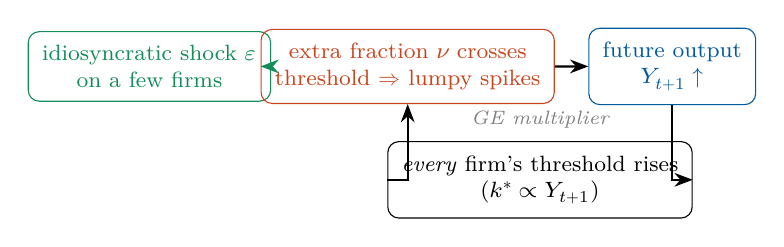
\begin{tikzpicture}[
		box/.style={draw, rounded corners, align=center, font=\footnotesize, inner sep=5pt},
		arr/.style={-{Stealth}, thick},
		scale=0.8
	]
		\node[box, shockc, draw=shockc] (shock) at (0,1.3) {idiosyncratic shock $\varepsilon$\\ on a few firms};
		\node[box, invest, draw=invest] (inv) at (4.1,1.3) {extra fraction $\nu$ crosses\\ threshold $\Rightarrow$ lumpy spikes};
		\node[box, accent, draw=accent] (Y) at (8.3,1.3) {future output\\ $Y_{t+1}\uparrow$};
		\node[box] (thr) at (6.2,-0.5) {\emph{every} firm's threshold rises\\ ($k^{*}\propto Y_{t+1}$)};
		\draw[arr, shockc] (shock) -- (inv);
		\draw[arr] (inv) -- (Y);
		\draw[arr] (Y.south) |- (thr);
		\draw[arr] (thr.west) -| (inv.south);
		\node[font=\scriptsize\itshape, gray] at (6.2,0.45) {GE multiplier};
	\end{tikzpicture}


	$$\text{Total induced inv.} = \sum_{i=1}^{\infty} \text{ induced fraction}^{(i)} \times \text{ average induced inv.}^{(i)}$$
	\begin{itemize}
		\item The induced fraction and average induced investing do not decay due to the lumpy investment assumption.
		\item With many firms, the idiosyncratic risk itself averages out, but the multiplied response does not. 
		
		$\implies$ Aggregate investment behaves as if hit by a common shock:
		\[\; I_t=\mu_{d,t}\,I_t^{*}.\]
	\end{itemize}
\end{frame}

\begin{frame}{The estimated DSGE model}
	% list the features of the model used in estimation, like sticky wage, investment adjustment cost, etc.
	Based on Smets and Wouters (2007), Herbst and Schorfheide (2015), augmented with the investment demand shock.
	\begin{itemize}
		\item \textbf{Nominal rigidities:} Calvo price setting; Erceg nominal wage rigidity.
		\item \textbf{Other frictions:} investment adjustment cost and endogenous capital utilization. 
		\item \textbf{Policy:} Taylor rule; output-stabilizing government spending.
		\item \textbf{Five structural shocks:} technology $\varepsilon_a$, IST $\varepsilon_s$, monetary $\varepsilon_R$, government $\varepsilon_g$, and investment demand $\varepsilon_d$.

	\end{itemize}
\end{frame}

\begin{frame}{Estimation: method and data}
	% 1. brief introduction on estimation method
	% 2. Data
	\begin{columns}[T,onlytextwidth]
		\column{0.5\textwidth}
		\textbf{Method}
		\begin{itemize}
			\item Bayesian estimation; methodology follows Smets and Wouters (2007),  Justiniano et al.\ (2010).
			\begin{itemize}
				\item Posterior via Metropolis--Hastings: $100{,}000$ draws.
			\end{itemize}
		\end{itemize}
		\column{0.5\textwidth}
		\textbf{Data}
		\begin{itemize}
			\item Six quarterly U.S.\ observables (FRED), \textbf{1983:Q1--2002:Q4}:
			\begin{itemize}\small
				\item output growth, CPI inflation, fed funds rate,
				\item hours, investment growth, gov.-spending growth.
			\end{itemize}
		\end{itemize}
	\end{columns}
\end{frame}

\begin{frame}{Baseline result: variance decomposition}
	% baseline result (FEVD)
	\textcolor{invest}{\textbf{ID shock}} alone explains $\approx\!\mathbf{29\%}$ of output and $\approx\!\mathbf{38\%}$ of investment FEVD.

	\vspace{1em}

	\centering
	\small
	\setlength{\tabcolsep}{1.0em}
	\begin{tabular}{l r r r r r r}
		\hline\hline
		Observable & $\varepsilon_g$ & \textcolor{accent}{$\varepsilon_{ist}$} & $\varepsilon_R$ & $\varepsilon_a$ & \textcolor{invest}{$\varepsilon_{id}$} & $\mathrm{meas}$ \\ 
		\hline
		Output & 2.47 & 31.47 & 3.88 & 31.67 & \textbf{29.03} & 1.48 \\ 
		Inflation & 0.41 & 12.67 & 10.15 & 63.11 & 11.96 & 1.70 \\ 
		Interest rate & 0.47 & 16.81 & 21.34 & 46.30 & 11.84 & 3.24 \\ 
		Hours & 3.07 & 40.36 & 3.94 & 9.19 & \textbf{36.16} & 7.27 \\ 
		Investment & 0.59 & 48.72 & 0.42 & 11.27 & \textbf{37.55} & 1.45 \\ 
		Gov. spending & 95.68 & 0.03 & 0.01 & 0.04 & 0.05 & 4.18 \\ 
		\hline
	\end{tabular}

	\vspace{0.4em}
	
	Frequency-domain FEVD (\%), business-cycle band \textbf{6--32} quarters (500 frequency bins).\\
	 $\varepsilon_g$ gov., \textcolor{accent}{$\varepsilon_s$ IST}, $\varepsilon_R$ monetary, $\varepsilon_a$ technology, \textcolor{invest}{$\varepsilon_d$ ID}.
\end{frame}

\begin{frame}{Baseline result: impulse responses}
	% baseline result (IRF) -- explain the IRF plot
	\centering
	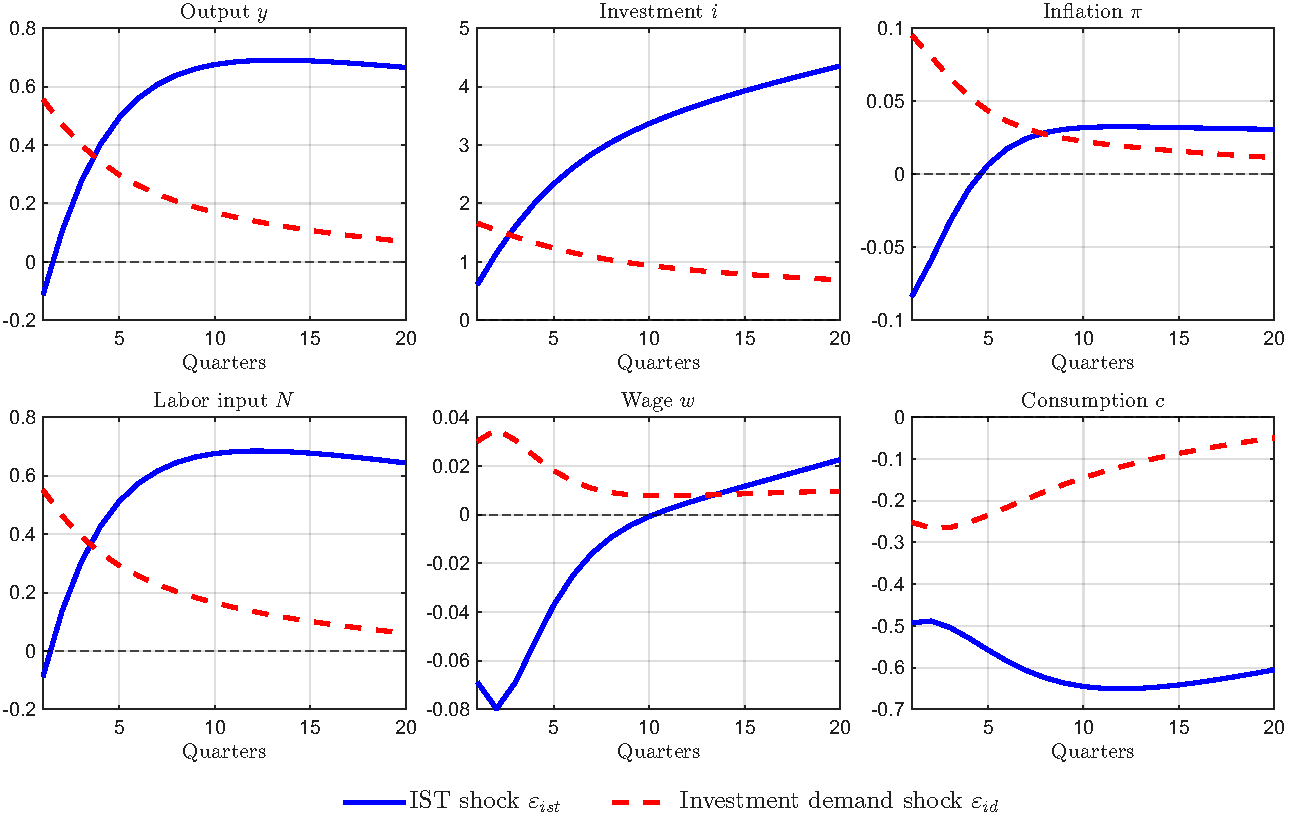
\includegraphics[width=0.77\textwidth]{compare_irf_delete_shock.pdf}
	\\[0.2em]
	\begin{columns}[T,onlytextwidth]
		\column{0.5\textwidth}
		\textcolor{accent}{\textbf{IST shock $\Rightarrow$ deflationary}}
		\begin{itemize}
			\item \textbf{Intertemporal substitution}: cheap investment $\Rightarrow$ save more today.
			\item labor supply shift dominates $\Rightarrow$ Wage $\downarrow$ while hours $\uparrow$.
		\end{itemize}
		\column{0.5\textwidth}
		\textcolor{invest}{\textbf{ID shock $\Rightarrow$ inflationary}}
		\begin{itemize}
			\item \textbf{Wealth effect}: higher future output raises lifetime wealth $\Rightarrow$ less impactful substitution effect.
			\item labor demand shift dominates  $\Rightarrow$ Wage $\uparrow$ and hours $\uparrow$.
		\end{itemize}
	\end{columns}
\end{frame}

\begin{frame}{Robustness: Smets--Wouters-style model}
	% FEVD and IRF of SW-type model
	\begin{itemize}
		\item Add habit formation, preference / price- / wage-markup shocks, and consumption and wage growth as observables.
		\item \textbf{ID shock turns marginal:} only $4.4\%$ of output and $13.6\%$ of investment FEVD.
	\end{itemize}
	\vspace{0.2em}
	\centering
	\footnotesize
	\begin{tabular}{l r r r r r r r r}
		\hline\hline
		Observable & $\varepsilon_g$ & \textcolor{accent}{$\varepsilon_{s}$} & $\varepsilon_R$ & $\varepsilon_a$ & $\varepsilon_b$ & $\varepsilon_p$ & $\varepsilon_w$ & \textcolor{invest}{$\varepsilon_{d}$} \\ 
		\hline
		Output & 6.15 & 10.31 & 7.86 & 43.58 & 17.21 & 5.00 & 5.52 & \textbf{4.37} \\ 
		Inflation & 0.05 & 1.78 & 0.82 & 18.85 & 0.40 & 53.05 & 25.04 & 0.00 \\ 
		Interest rate & 0.19 & 7.16 & 30.37 & 26.67 & 4.51 & 10.39 & 20.72 & 0.00 \\ 
		Hours & 2.00 & 20.43 & 7.10 & 34.85 & 7.86 & 1.10 & 26.35 & 0.30 \\ 
		Investment & 0.25 & 54.98 & 2.43 & 18.59 & 3.19 & 0.62 & 6.33 & \textbf{13.62} \\ 
		Wage & 0.00 & 0.12 & 0.14 & 18.25 & 0.30 & 16.96 & 64.23 & 0.00 \\ 
		Consumption & 0.25 & 2.36 & 6.48 & 43.49 & 42.01 & 1.92 & 3.49 & 0.00 \\ 
		Gov. spending & 99.90 & 0.01 & 0.01 & 0.05 & 0.02 & 0.01 & 0.01 & 0.00 \\ 
		\hline
	\end{tabular}
	\\[0.4em]
	{\scriptsize Unconditional FEVD (\%): Smets--Wouters-style model. $\varepsilon_g$ gov., \textcolor{accent}{$\varepsilon_s$ IST}, $\varepsilon_R$ monetary, $\varepsilon_a$ technology, $\varepsilon_b$ preference, $\varepsilon_p$ price-markup, $\varepsilon_w$ wage-markup, \textcolor{invest}{$\varepsilon_d$ ID}.}
\end{frame}

\begin{frame}{Takeaway}
	% Conclusion
	\begin{itemize}
		\item Revisits investment-side shocks by testing \textbf{investment demand shock} in an estimated DSGE model.
		\item \textbf{Baseline:} the ID shock alone explains $\approx 40\%$ of output and $\approx 50\%$ of investment FEVD---a competitive driver---and generates an inflationary expansion with comovement (vs.\ deflationary IST).
		\item \textbf{Limitations:}
		\begin{itemize}
			\item results are specification-sensitive: the SW-style model shrinks the ID shock.
			\item no direct data identifies the ID shock---identification leans on comovement differences, hard to test over the whole parameter space;
			\item imperfect fit and some extreme posteriors in the baseline;
		\end{itemize}
	\end{itemize}
\end{frame}

\appendix
\begin{frame}[c]{}
	\centering
	{\Large\textbf{Backup: toy model details}}
\end{frame}

\begin{frame}{From idiosyncratic shock to investment demand shock}
	The reduced-form investment demand shock $\mu_{d,t}$:
		\[
			I_t=\mu_{d,t}\,I_t^{*},\quad
			\ln\mu_{d,t}=(1-\rho_d)\ln\mu_d+\rho_d\ln\mu_{d,t-1}+\varepsilon_{d,t}.
		\]

	\vspace{0.5em}

	\textbf{Intuition:} Firms decide their investment according to the its own \textbf{productivity} and \textbf{aggregate output}; (i) if some firms receive positive productivity shock, they will increase their investment; (ii) the increase in investment means more future output; (iii) thus firms not influenced by the shock will also invest more.
	\vspace{1em}

	Standard New-Keynesian CES aggregator and demand; $a_{j,t}\in\{a_L,a_H\}$ is deterministic:
	\[
		Y_t=\Big(\int_0^1 y_{j,t}^{\frac{\eta-1}{\eta}}\,dj\Big)^{\frac{\eta}{\eta-1}},
		\quad
		y_{j,t}=\Big(\frac{p_{j,t}}{P_t}\Big)^{-\eta}Y_t,
		\quad
		y_{j,t}=a_{j,t}k_{j,t}.
	\]
	Combining demand and production, real revenue is
	\[
		r_{j,t}(a_{j,t},k_{j,t})=\frac{p_{j,t}y_{j,t}}{P_t}
		=\big(a_{j,t}k_{j,t}\big)^{1-\frac1\eta}\,Y_t^{\frac1\eta}.
	\]
	\begin{itemize}\small
		\item Concave in own capital ($\eta>1$): diminishing returns through the demand curve.
	\end{itemize}
\end{frame}

\begin{frame}{Lumpy investment and the investment threshold}
	% --- top region: text (left) + figure pinned NE (right) ---
	\begin{columns}[T,onlytextwidth]
		\column{0.5\textwidth}
		\vspace{0.2em}
		Firms solve
		\[
			\max_{\{i_{t+\tau}\}}\ \underbrace{\sum_{\tau\ge0}\Lambda_{t,t+\tau}\big(r_{j,t+\tau}-i_{j,t+\tau}\big)}_{\coloneq V},
		\]
		$$\begin{aligned}
			\text{s.t. }&k_{j,t+\tau+1}=(1-\delta)k_{j,t+\tau}+i_{j,t+\tau},\\
			&i_{j,t+\tau}\in\{0,\ (\lambda-1)(1-\delta)k_{j,t+\tau}\},\\
			&\lambda>1.
		\end{aligned}$$

		\column{0.5\textwidth}
		\vspace{-0.6em}
		\centering
		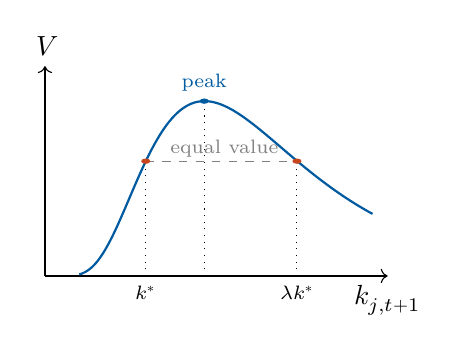
\begin{tikzpicture}[xscale=1.28,yscale=0.74]
			% axes
			\draw[->] (0,0) -- (3.4,0) node[below]{$k_{j, t+1}$};
			\draw[->] (0,0) -- (0,3.6) node[above]{$V$};
			% hump: peak at sqrt(lambda)*k*, k*=1, lambda=2.5 -> peak 1.58
			\draw[thick,accent,domain=0.34:3.25,samples=140,smooth,variable=\x]
				plot ({\x},{3*exp(-2*(ln(\x)-0.459)^2)});
			% equal-value horizontal line between k* and lambda k*
			\draw[dashed,gray] (1,1.97) -- (2.5,1.97);
			\draw[dotted] (1,0) -- (1,1.97);
			\draw[dotted] (2.5,0) -- (2.5,1.97);
			\draw[dotted] (1.58,0) -- (1.58,3.0);
			% points
			\fill[invest] (1,1.97) circle (1.3pt);
			\fill[invest] (2.5,1.97) circle (1.3pt);
			\fill[accent] (1.58,3.0) circle (1.3pt);
			% x ticks
			\node[below,font=\scriptsize] at (1,0) {$k^{*}$};
			\node[below,font=\scriptsize] at (2.5,0) {$\lambda k^{*}$};
			\node[above,font=\scriptsize,accent] at (1.58,3.0) {peak};
			\node[font=\scriptsize,gray] at (1.78,2.18) {equal value};
		\end{tikzpicture}
	\end{columns}

	% --- bottom region: full-width text wrapping under the figure ---
	\vspace{0.3em}
	Indifference at $k^*$ pins down the threshold:
	\[
		k_{j,t+1}^{*}=a_{j,t+1}^{\,\eta-1}\,\Phi_t(\Lambda_t, \Lambda_{t+1})\,Y_{t+1}
	\]
	
	\vspace{0.4em}
	Normalize a firm's position by its \textbf{distance to the threshold}
	\[
		s_{j,t+1}=\frac{\log\!\big(k_{j,t+1}/k_{j,t+1}^{*}\big)}{\log\lambda}\implies
		i_{j,t}=
		\begin{cases}
			(\lambda-1)(1-\delta)k_{j,t}, & s_{j,t+1}<0\\
			0, & s_{j,t+1} \geq 0
		\end{cases}
	\]
\end{frame}


\begin{frame}{(i): Idiosyncratic shock $\to$ investing fraction}
	% --- top region: text (left) + figure pinned NE (right) ---
	\vspace{1em}
	\begin{columns}[T,onlytextwidth]
		\column{0.61\textwidth}

		Without investing, under stationary distribution ($Y = Y_t = Y_{t+1}$, $\Phi = \Phi_t = \Phi_{t+1}$), $s_{j,t+1}$ drifts:
		\[
		\begin{aligned}
		s_{j,t+1} = &s_{j,t} \\
		&-\underbrace{\frac{-\log(1-\delta)+(\eta-1)\log\left(a_{t+1}/a_t\right)}{\log\lambda}}_{\coloneq s^{*}(a_t,a_{t+1})}
		\end{aligned}
		\]

		\column{0.39\textwidth}
		\centering
		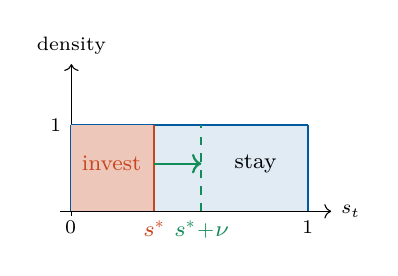
\begin{tikzpicture}[xscale=3,yscale=1.1]
			% axis
			\draw[->] (-0.05,0) -- (1.1,0) node[right,font=\scriptsize]{$s_t$};
			\draw[->] (0,-0.05) -- (0,1.7) node[above,font=\scriptsize]{density};
			% uniform density box on [0,1)
			\fill[accent!12] (0,0) rectangle (1,1);
			\draw[accent,thick] (0,1) -- (1,1);
			\draw[accent,thick] (0,0)--(0,1);
			\draw[accent,thick] (1,0)--(1,1);
			% investing region [0,s*]
			\fill[invest!30] (0,0) rectangle (0.35,1);
			\draw[invest,thick] (0.35,0)--(0.35,1);
			\node[invest,font=\footnotesize,below] at (0.35,0) {$s^{*}$};
			% epsilon shifted threshold
			\draw[shockc,thick,->] (0.35,0.55)--(0.55,0.55);
			\draw[shockc,thick,dashed] (0.55,0)--(0.55,1);
			\node[shockc,font=\footnotesize,below] at (0.55, 0) {$s^{*}\!+\!\nu$};
			% labels
			\node[invest,font=\footnotesize] at (0.17,0.55) {invest};
			\node[font=\footnotesize] at (0.78,0.55) {stay};
			\node[below,font=\scriptsize] at (0,0) {$0$};
			\node[below,font=\scriptsize] at (1,0) {$1$};
			\node[left,font=\scriptsize] at (0,1) {$1$};
		\end{tikzpicture}
	\end{columns}

	% --- bottom region: full-width text wrapping under the figure ---
	\vspace{1em}

	\textbf{Assume} $s_t\mid a_t\sim U[0,1)$ under stationary distribution.

	\vspace{1em}

	\begin{itemize}
		\item Then $s^{*}(a_t,a_{t+1}) \times 1$ is the \textbf{stationary investing fraction}
		\item Add an $i.i.d.$\ shock $\varepsilon$ on $a_{t+1}$ for the firms in group $(a_t = b, a_{t+1} = b')$:
		\[
			s^{*}(b,\varepsilon b')=s^{*}(b,b')+\underbrace{\frac{(\eta-1)\log\varepsilon}{\log\lambda}}_{\coloneq \nu}.
		\]
		\item The cutoff in that group rises by $\nu$, so an extra $\nu \times 1$ fraction invests.
	\end{itemize}
\end{frame}

\begin{frame}{(ii)\&(iii): Investing fraction $\to$ aggregate output $\to$ investing fraction}
	% --- top region: text (left) + figure pinned NE (right) ---
	\begin{columns}[T,onlytextwidth]
		\column{0.8\textwidth}
		More investment in $(b,b')$ raises \textbf{future output} of this group, which is a part of future aggregate output:
		\[\begin{aligned}
			Y_{t+1}(b, b', \nu)
			=\Big(\omega(b,b')\!\!\int_{0}^{s^*+\nu}\!\! \big(b'\lambda (1-\delta) k_{t}(s_t)\big)^{\frac{\eta-1}{\eta}}\,dF(s_t\mid b)& \\
			+ \text{no investment firms}\Big)^{\frac{\eta}{\eta-1}}&
		\end{aligned}
		\]

		\column{0.2\textwidth}
		\vspace{-0.3em}
		\centering
		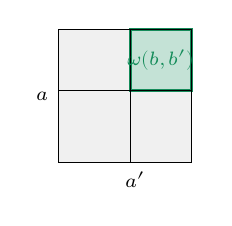
\begin{tikzpicture}[scale=0.65]
			% 2x2 groups, sizes ~ omega
			\fill[gray!12] (0,0) rectangle (1.4,1.4);
			\fill[gray!12] (1.4,0) rectangle (2.6,1.4);
			\fill[gray!12] (0,1.4) rectangle (1.4,2.6);
			% highlight shocked group (b,b'): a=H (top), a'=H (right)
			\fill[shockc!25] (1.4,1.4) rectangle (2.6,2.6);
			\draw[shockc,very thick] (1.4,1.4) rectangle (2.6,2.6);
			% grid
			\draw (0,0) rectangle (2.6,2.6);
			\draw (1.4,0)--(1.4,2.6);
			\draw (0,1.4)--(2.6,1.4);
			% labels of omega

			\node[font=\scriptsize,shockc] at (2.0,2.0) {$\omega(b,b')$};
			% axis labels
			\node[below,font=\scriptsize] at (1.5,0) {$a'$};
			\node[left,font=\scriptsize] at (0,1.3) {$a$};
		\end{tikzpicture}
	\end{columns}

	% --- bottom region: full-width text wrapping under the figure ---
	\vspace{0.5em}
	\begin{itemize}
		\item Higher $Y_{t+1}$ shifts the cutoff in every group, and induce an extra investing fraction:
		\[
		\begin{aligned}
			\nu^{(1)}(a, a') = \frac{\log (Y_{t+1}(\nu)/ Y_{t+1}(0))}{\log\lambda},\quad \nu^{(1)}\coloneq \sum_{(a,a')}\omega(a,a')\,\nu^{(1)}(a, a').
		\end{aligned}
		\]
		\item The first $\nu$ of investing firms raises $Y$, which induces $\nu^{(1)}$ more, which raises $Y$ again $\dots$ a GE multiplier that iterates to a new equilibrium.
	\end{itemize}
\end{frame}

\begin{frame}{Total induced investment $\gg \nu$}
	$$\text{Total induced inv.} = \sum_{i=1}^{\infty} \text{ induced fraction}^{(i)} \times \text{ average induced inv.}^{(i)}$$

	\begin{itemize}
		\item \textbf{Scale of induced fraction}
		\[
		 \lim_{\nu\to 0}\frac{\nu^{(1)}}{\omega(b,b')\,\nu}=1\
		\]
		
		The $\nu^{(1)}$ has the \textbf{same scale} as the original fraction 
			
		$\implies$ each $\omega(a, a') \nu^{(1)}(a, a')$ will induce the same scale $\nu^{(2)}(\nu^{(1)}(a, a'))$ again.

		\vspace{0.2em}

		\item \textbf{Scale of average induced investment}
		\[
			\frac{\partial \Delta x(a, a', \nu)}{\partial \nu}\Big|_{\nu=0} = (\lambda - 1)(1-\delta) \lambda^{s^*} a^{\eta - 1}\Psi Y
		\]
		
		The derivative says $\Delta x(a, a', \nu) = O(\nu)$.
		
		$\implies$ average induced investment will not decay faster than $\nu$.
	\end{itemize}
\end{frame}
\end{document}
